\lstset{language=VBScript,
        basicstyle=\footnotesize\ttfamily,
        breaklines=true,
        tabsize=2,
        numbers=left,
        numberstyle=\tiny,
        numbersep=7pt,
        showspaces=false,
        keywordstyle=\color{Blue}\textbf,
        commentstyle=\color{Red}\emph,
        showstringspaces=false,
        stringstyle=\color{BurntOrange}
        }
\section{Instrukcja użytkownika}
%\subsection{Specyfikacja zewnętrzna}

\subsection{Ekrany powitalne}

\noindent Po uruchomieniu aplikacji pierwszym widocznym oknem, będzie ekran powitalny (Rys.~\ref{splash_screen}). U~jego dołu wyświetlony jest przebieg kontroli systemu wykonywanej każdorazowo przy~próbie włączenia programu. Podczas testu sprawdzane są:
\begin{enumerate}
\item istnienie poprawnej bazy danych i~możliwość połączenia,
\item istnienie portów szeregowych,
\item dostęp do wszystkich potrzebnych sterowników.
\end{enumerate}
\noindent W~razie potrzeby automatycznie uzupełniane~są słowniki konieczne dla poprawnego działania aplikacji.

\begin{figure}[!htb]
\centering 		
  \subfloat[Windows]{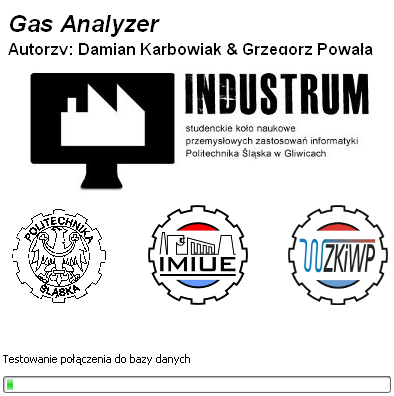
\includegraphics[width=0.45\textwidth]{images/splashScreenW}}   
  \hspace{2mm}          
  \subfloat[Linux]{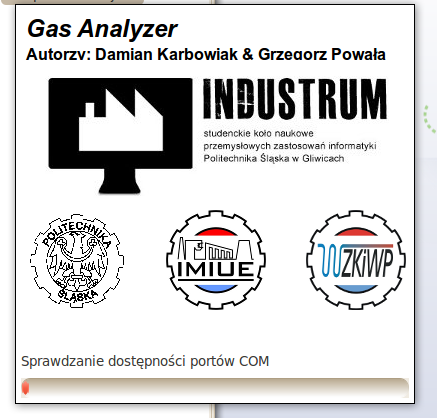
\includegraphics[width=0.45\textwidth]{images/splashScreenL}}
\caption{Okno ładowania} 	
\label{splash_screen}
\end{figure}

\noindent W~przypadku wykrycia braku elementów niezbędnych do poprawnego działania programu wyświetlony zostanie odpowiedni komunikat (Rys.~\ref{dbError} i Rys.~\ref{rxtxError}).

\begin{figure}[!htb]
\centering 		
  \subfloat[Windows]{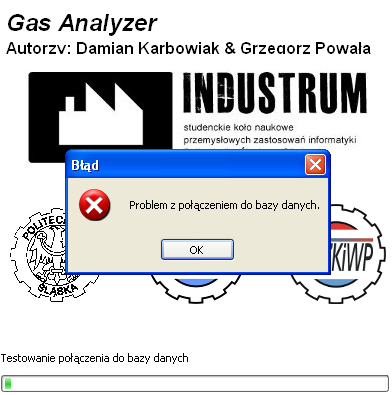
\includegraphics[width=0.35\textwidth]{images/dbErrorW}}    
  \hspace{2mm}
  \subfloat[Linux]{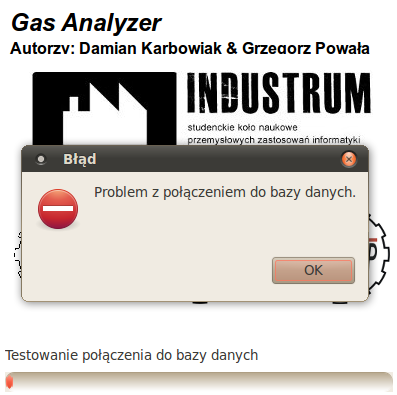
\includegraphics[width=0.35\textwidth]{images/dbErrorL}}
\caption{Komunikat o błędzie łączenia do bazy danych} 	
\label{dbError}
\end{figure}

\begin{figure}[!htb]
\centering 		
  \subfloat[Windows]{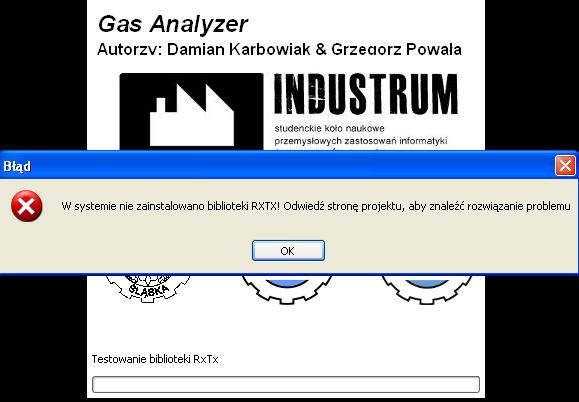
\includegraphics[width=0.45\textwidth]{images/rxtxErrorW}}    
  \hspace{2mm}
  \subfloat[Linux]{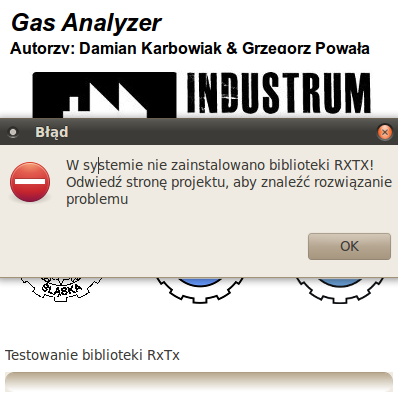
\includegraphics[width=0.45\textwidth]{images/rxtxErrorL}}
\caption{Okno błędu braku biblioteki RXTX} 	
\label{rxtxError}
\end{figure}

\noindent Po wykonaniu wszystkich testów i~sprawdzeniu poprawności konfiguracji systemu użytkownik zostaje przeniesiony do głównego okna aplikacji (Rys.~\ref{main}). Bezpośrednio po uruchomieniu większość funkcji jest nieaktywna. W~celu ich uaktywnienia konieczne jest utworzenie bądź wczytanie istniejącego pomiaru. Operacje te są opisane w~dalszej części instrukcji. W~tym momencie można zaobserwować budowę programu. Na~górze okna widoczne są menu.
\begin{itemize}
\item Menu ,,Plik'': umożliwia rozpoczęcie (,,Nowy pomiar'') i~wczytanie poprzedniego (,,Otwórz pomiar"'') pomiaru oraz wyłączenie aplikacji (,,Wyjście'').
\item Menu ,,Edycja'': umożlwia edycję wszelkich parametrów pomiaru. Zaliczają się do nich:
\begin{itemize}
\item ,,Edytuj prowadzących pomiar'': umożliwia edycję danych o~osobach przeprowadzających pomiar. Prócz danych personalnych przechowywane są informacje o tytule naukowym i~pełnionej funkcji (Rys.~\ref{editUser}),

\begin{figure}[!htb]
\centering 		
  \subfloat[Windows]{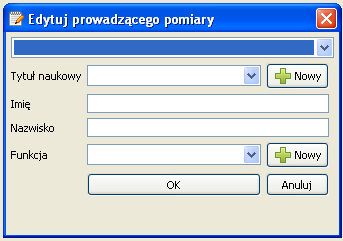
\includegraphics[width=0.45\textwidth]{images/editUserW}}    
  \hspace{2mm}
  \subfloat[Linux]{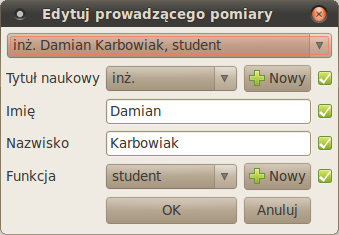
\includegraphics[width=0.45\textwidth]{images/editUserL}}
\caption{Okno edycji danych użytkownika} 	
\label{editUser}
\end{figure}

\item ,,Edytuj tytuły'': umożliwia edycję tytułów naukowych (Rys.~\ref{editUser}),
\item ,,Edytuj funkcje'': umożliwia edycję funkcji, które są przypisane użytkownikom pomiaru np. ,,prowadzący pomiar'', ,,obserwator'', ,,kontroler'', ,,student'' (Rys.~\ref{editUser}),
\item ,,Edytuj miejsca'': umożliwia edycję informacji o miejscu, w którym odbywa się pomiar (Rys.~\ref{editUser}),
\item ,,Edytuj obiekty'': umożliwia edycję obiektów będących przedmiotem pomiaru (Rys.~\ref{editUser}),
\end{itemize}
\item Menu ,,Pomiar'':
\item Menu ,,Sieć'':
\item Menu ,,Pomoc'':
\end{itemize}

\begin{tikzpicture}
\node[color=black,draw=white,fill=uwaga,shape=rectangle,rounded corners=0.5ex,
text width=36em, text centered] at (4,0) 
{
\textbf{UWAGA}\linebreak
W~celu wykonania pomiaru konieczne jest uzupełnienie informacji o~minimum jednym użytkowniku oraz o~przynajmniej jednym obiekcie będącym przedmiotem pomiaru. W~ramach jednego miejsca może istnieć wiele obiektów.
};
\end{tikzpicture}

\begin{figure}[!htb]
\centering 		
  \subfloat[Windows]{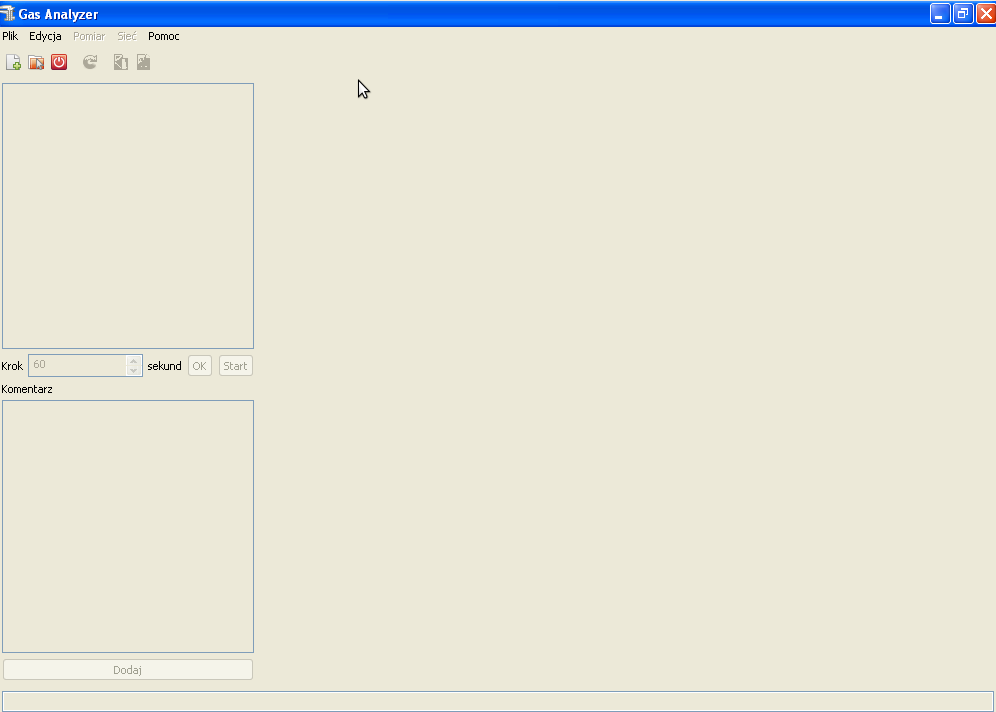
\includegraphics[width=0.45\textwidth]{images/mainW}}   
  \hspace{2mm}          
  \subfloat[Linux]{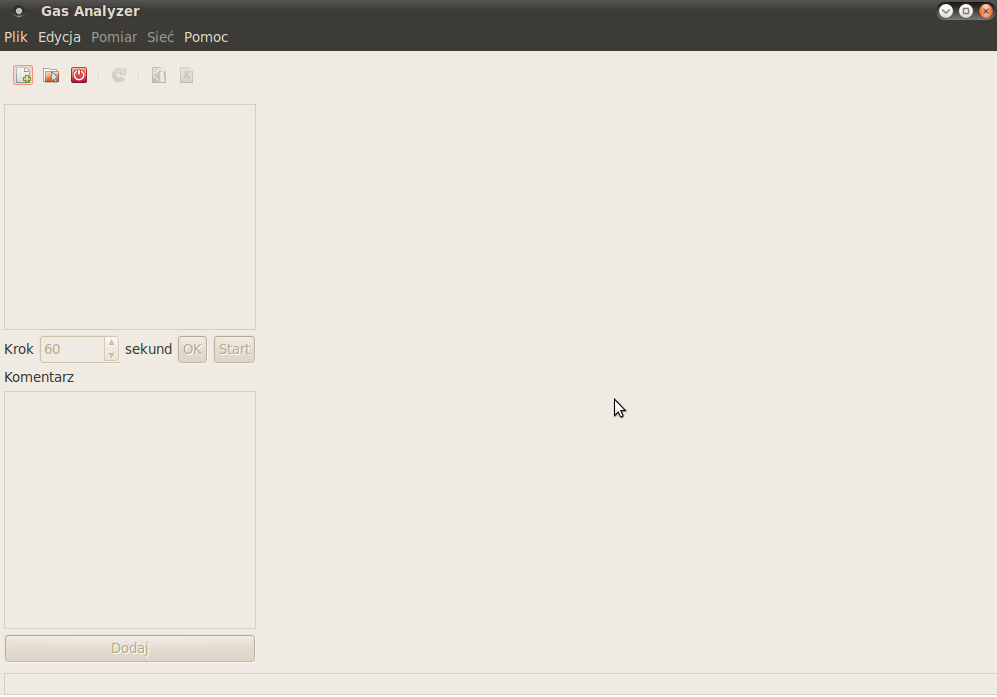
\includegraphics[width=0.45\textwidth]{images/mainL}}
\caption{Okno główne} 	
\label{main}
\end{figure}

\begin{figure}[!htb]
\centering 		
  \subfloat[Windows]{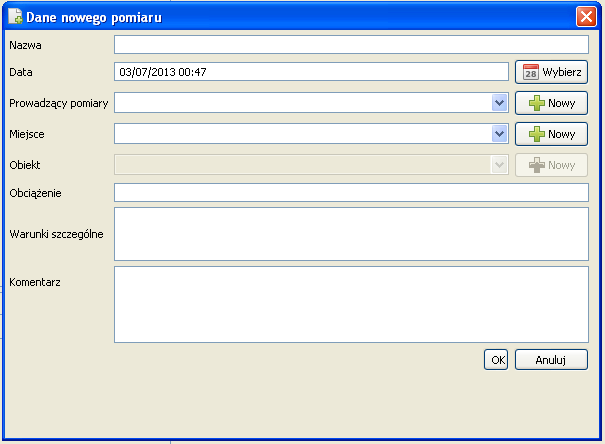
\includegraphics[width=0.45\textwidth]{images/newSurveyW}}                
  \hspace{2mm}
  \subfloat[Linux]{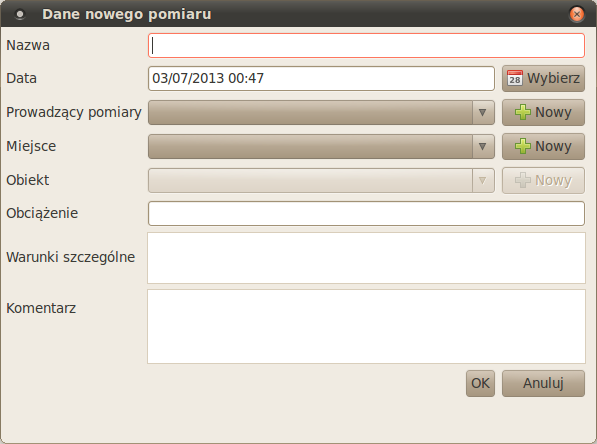
\includegraphics[width=0.45\textwidth]{images/newSurveyL}}
\caption{Dodawanie nowego pomiaru} 	
\label{main}
\end{figure}

\begin{figure}[!htb]
\centering 		
  \subfloat[Windows]{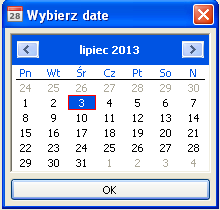
\includegraphics[width=0.25\textwidth]{images/calendarW}}    
  \hspace{2mm}
  \subfloat[Linux]{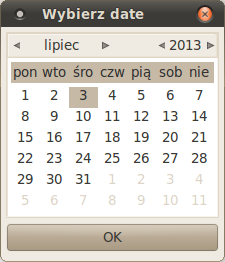
\includegraphics[width=0.25\textwidth]{images/calendarL}}
\caption{Okno wyboru daty} 	
\label{main}
\end{figure}

\begin{figure}[!htb]
\centering 		
  \subfloat[Windows]{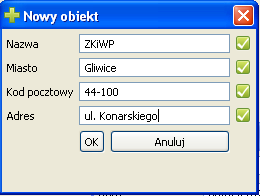
\includegraphics[width=0.45\textwidth]{images/newPlaceW}}                
  \hspace{2mm}
  \subfloat[Linux]{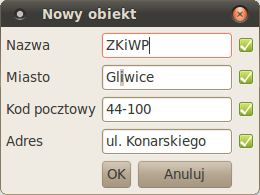
\includegraphics[width=0.45\textwidth]{images/newPlaceL}}
\caption{Dodawanie nowego miejsca} 	
\label{main}
\end{figure}

\begin{figure}[!htb]
\centering 		
  \subfloat[Windows]{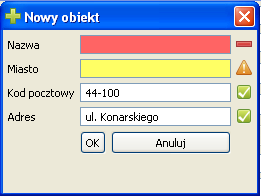
\includegraphics[width=0.45\textwidth]{images/newPlaceErrorW}}                
  \hspace{2mm}
  \subfloat[Linux]{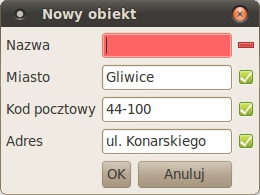
\includegraphics[width=0.45\textwidth]{images/newPlaceErrorL}}
\caption{Błąd przy dodawaniu nowego miejsca} 	
\label{main}
\end{figure}

\begin{figure}[!htb]
\centering 		
  \subfloat[Windows]{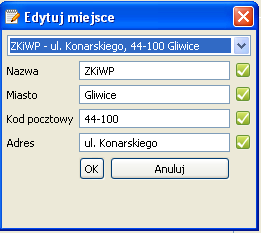
\includegraphics[width=0.45\textwidth]{images/editPlaceW}}                
  \hspace{2mm}
  \subfloat[Linux]{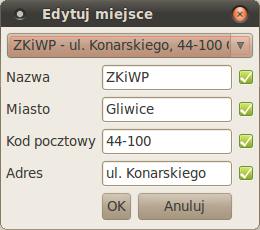
\includegraphics[width=0.45\textwidth]{images/editPlaceL}}
\caption{Edytowanie istniejącego miejsca} 	
\label{main}
\end{figure}

\begin{figure}[!htb]
\centering 		
  \subfloat[Windows]{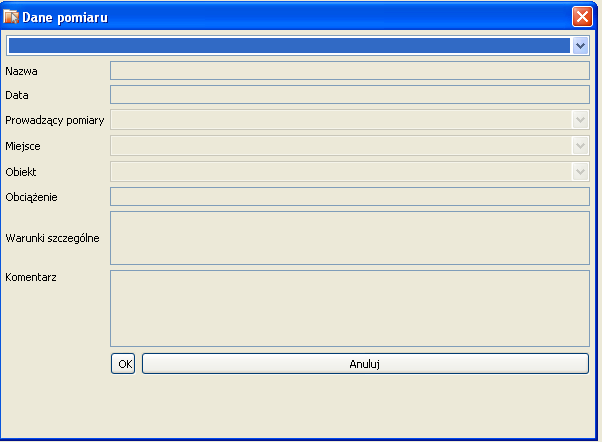
\includegraphics[width=0.45\textwidth]{images/openSurveyW}}                
  \hspace{2mm}
  \subfloat[Linux]{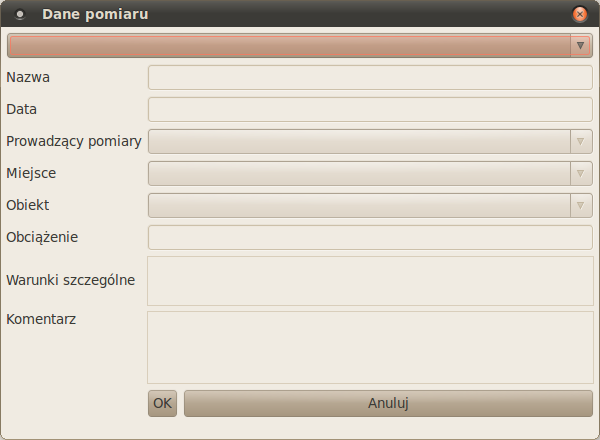
\includegraphics[width=0.45\textwidth]{images/openSurveyL}}
\caption{Otwieranie istniejącego pomiaru} 	
\label{main}
\end{figure}

\begin{figure}[!htb]
\centering 		
  \subfloat[Windows]{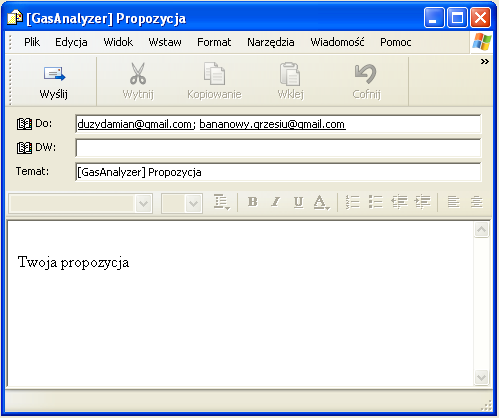
\includegraphics[width=0.45\textwidth]{images/suggestionW}}                
  \hspace{2mm}
  \subfloat[Linux]{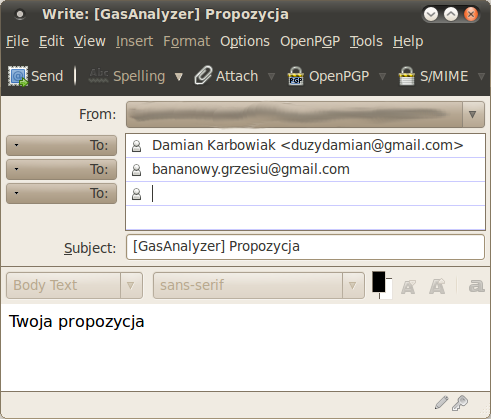
\includegraphics[width=0.45\textwidth]{images/suggestionL}}
\caption{Wysyłanie sugestii} 	
\label{main}
\end{figure}